\def\snip{
    Từ những thí nghiệm trong \textit{phần 3.1}, nhóm tác giả đã đưa ra đề xuất phương pháp chuẩn bị dữ liệu Scale Normalization for Image Pyramids (gọi tắt là SNIP) \cite{singh2018analysis}.
    Phương pháp SNIP hướng đến việc sử dụng tối đa sự đa dạng trong biến thể của đối tượng trong bộ dữ liệu trong khi có thể thu hẹp được sự biến động trong kích thước của các đối tượng.
    Từ đó, mô hình sẽ có nhiều dữ liệu nhất có thể và cũng sẽ có kích thước đối tượng phù hợp nhất để học.
    Ý tưởng chung của SNIP dựa trên \textit{image pyramid} đã được nhắc đến trong phần \textit{phần 2.2. Kiến trúc Feature Pyramid Networks}.

    \noindent
    \textbf{\textit{Ý tưởng của phương pháp chuẩn bị dữ liệu SNIP}} \\
    Một điểm yếu của việc chuẩn bị dữ liệu MST ở thí nghiệm \textit{phần 3.1} là việc một ảnh bất kỳ được huấn luyện với nhiều kích thước khác nhau khiến cho khi ảnh đó ở kích thước lớn (1400x2000) thì các đối tượng lớn sẽ trở nên khó khăn cho mô hình.
    Điều này diễn ra tương tự đối với các đối tượng nhỏ khi ảnh đó ở kích thước nhỏ (480x800).

    \begin{figure}[H]
        \centering
        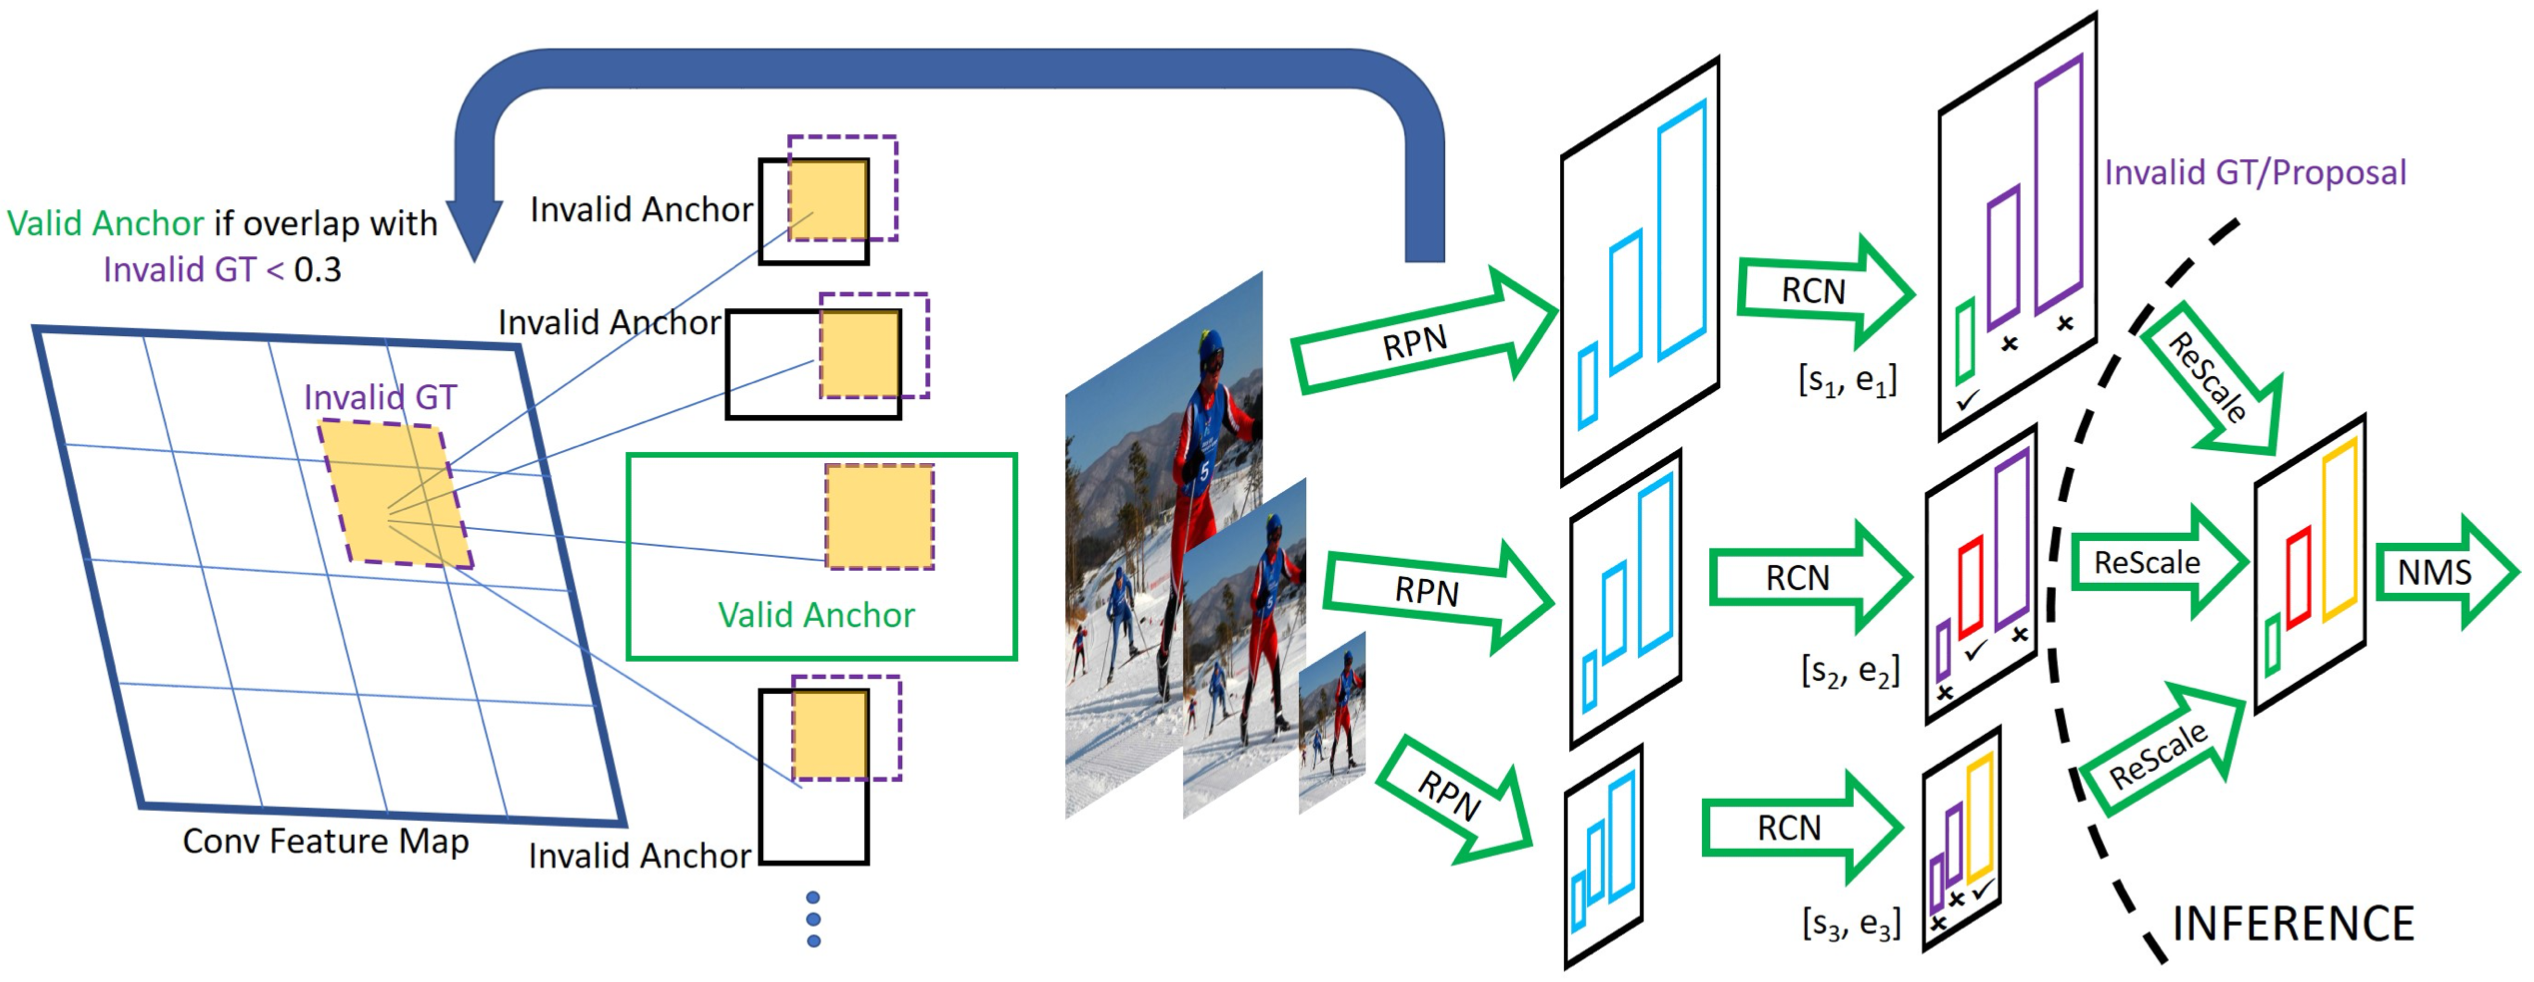
\includegraphics[width=16cm] {images/snip_model}
        \caption{Chi tiết kiến trúc phương pháp chuẩn bị dữ liệu SNIP trong quá trình huấn luyện và test (Nguồn: \cite{singh2018analysis})}
        \label{fig:snip_model}
    \end{figure}

    \noindent
    phương pháp chuẩn bị dữ liệu SNIP được coi là một phiên bản nâng cấp hơn của MST.
    Ý tưởng chính của SNIP là trong quá trình huấn luyện, các đối tượng có kích thước tương đồng với bộ dữ liệu pretrained của mô hình (thông thường là 224x224) sẽ được sử dụng để huấn luyện và loại bỏ các đối tượng, mà sau khi thay đổi kích thước ảnh, trở nên quá lớn hoặc quá nhỏ.

    \noindent
    \textbf{\textit{Kết quả của mô hình khi sử dụng phương pháp chuẩn bị dữ liệu SNIP}} \\
    Kết quả của mô hình khi sử dụng phương pháp chuẩn bị dữ liệu SNIP so sánh với các thí nghiệm khác trong \textit{phần 3.1} được thể hiện ở hình \ref{fig:snip_results_1}.
    Việc sử dụng SNIP giúp mô hình đạt độ chính xác cao hơn so với các mô hình sử dụng các phương pháp chuẩn bị dữ liệu khác.

    \noindent
    Nhóm tác giả cũng so sánh kết kết quả của các mô hình sử dụng và không sử dụng phương pháp chuẩn bị dữ liệu SNIP cùng các kiến trúc backbone khác nhau.
    Các mô hình sử dụng trong thí nghiệm là D-RFCN \cite{}, Mask-RCNN \cite{}, G-RMI \cite{}, Faster-RCNN \cite{}.
    Kỹ thuật được bổ sung trong một số cấu hình là RCN \cite{}.
    Các cấu hình sử dụng phương pháp chuẩn bị dữ liệu SNIP có ký hiệu \textit{+ SNIP}.
    Chi tiết các backbone sử dụng trong mỗi cấu hình được chú thích ở cột \textit{Backbone}.
    
    \begin{figure}[H]
        \centering
        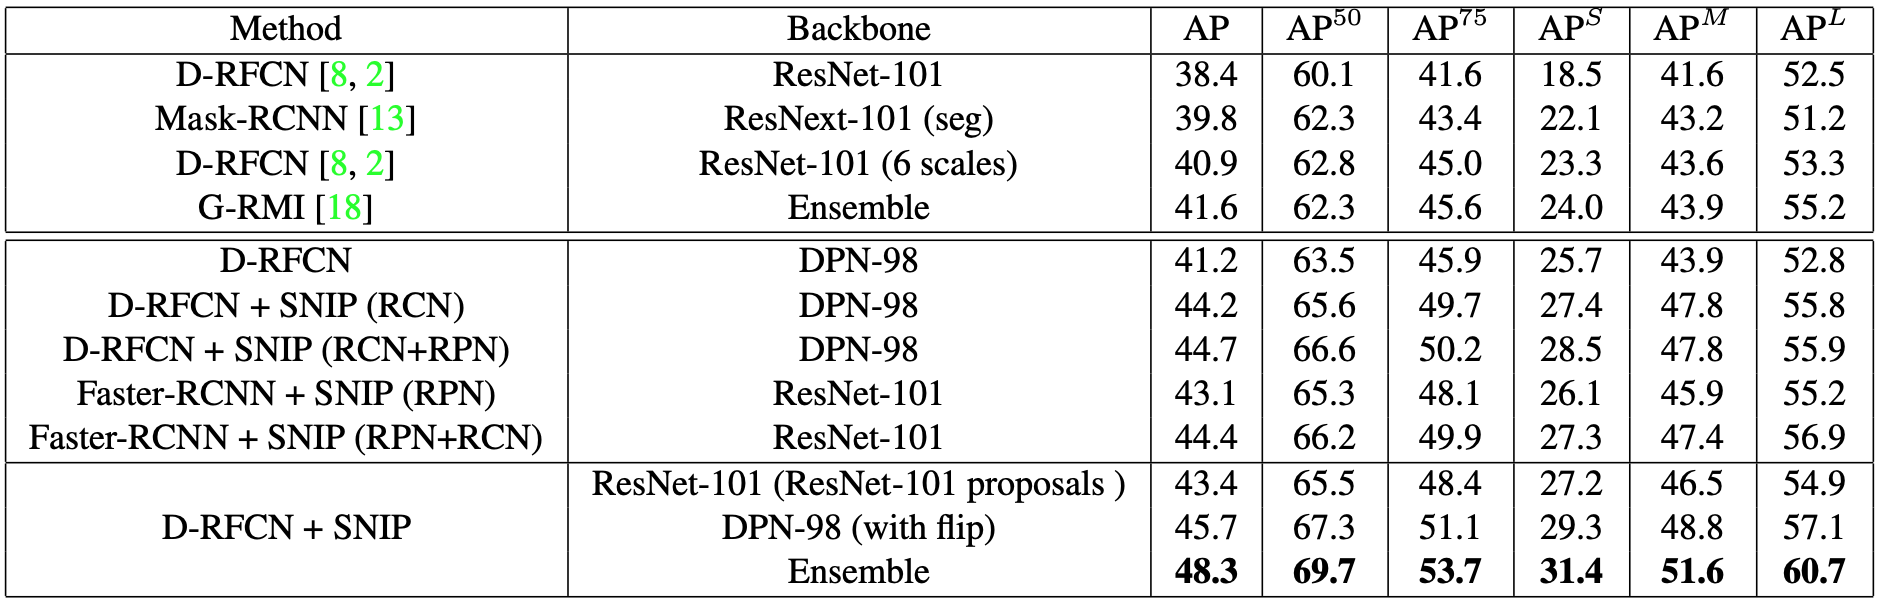
\includegraphics[width=16cm] {images/snip_results_2}
        \caption{Kết quả của các mô hình sử dụng và không sử dụng phương pháp chuẩn bị dữ liệu SNIP (Nguồn: \cite{singh2018analysis})}
        \label{fig:snip_results_2}
    \end{figure}

    \noindent
    Kết quả của mô hình D-RFCN sử dụng SNIP và backbone Ensemble đạt chỉ số cao hơn khá nhiều so với các cấu hình khác.
    Ngoài ra, các cấu hình sử dụng SNIP cũng đạt chỉ số cao hơn các cấu hình không sử dụng SNIP.
    Điều này chứng minh được vai trò của phương pháp chuẩn bị dữ liệu SNIP đối với các mô hình object detection.

    \noindent
    \textbf{\textit{Vấn đề tồn đọng của phương pháp chuẩn bị dữ liệu SNIP}} \\
    Tuy rằng đã có những cải thiện trong kết quả của các mô hình sử dụng phương pháp chuẩn bị dữ liệu SNIP, nhưng nhóm tác giả vẫn nêu ra những vấn đề tồn đọng là lãng phí chi phí tính toán trong quá trình huấn luyện.
    Cụ thể, những đối tượng có kích thước lớn và bị loại bỏ trong quá trình huấn luyện, nhưng các lớp Conv \index{lớp Conv} vẫn phải tính toán trên các phần này dẫn đến sự lãng phí tài nguyên tính toán.
}